\section{道路同伦}
\label{section:ch09-sec51}

我们始终假定读者熟悉商拓扑 (第 22 节) 和局部连通性 (第 25 节).

在定义空间 $X$ 的基本群之前, 我们考虑 $X$ 中的道路以及道路之间的一个等价关系"道路同伦", 并且还将在这些等价类构成的集合中定义一种运算, 使得这个等价类的集合成为代数学中所说的一个广群.

\begin{definition}[同伦]
\label{definition:ch09-sec51-homotopy}
设 $f$ 和 $f'$ 是从空间 $X$ 到空间 $Y$ 的两个连续映射. 我们说 $f$ \textbf{同伦于} $f'$, 如果有一个连续映射 $F\colon X\times I\to Y$ 使得对于每一个 $x$,
\[
F(x,0)=f(x)\quad\text{和}\quad F(x,1)=f'(x).
\]
(其中 $I=[0,1]$.) 映射 $F$ 称为是 $f$ 和 $f'$ 之间的一个\textbf{同伦}(homotopy). 如果 $f$ 同伦于 $f'$, 则记作 $f\simeq f'$. 如果 $f\simeq f'$ 并且 $f'$ 是一个常值映射, 则称 $f$ 是\textbf{零伦的}(nulhomotopic).
\end{definition}

我们将一个同伦设想为从 $X$ 到 $Y$ 的映射的一个连续单参数族, 如果把参数 $t$ 想象为时间变量, 那么当 $t$ 从 $0$ 变到 $1$ 时, 同伦 $F$ 便将映射 $f$ 连续地"形变"为映射 $f'$.

现在考虑 $f$ 是 $X$ 中的一条道路这种特殊情形. 重申下述定义: 如果 $f\colon[0,1]\to X$ 是一个连续映射, 使得 $f(0)=x_0$, $f(1)=x_1$, 则称 $f$ 是 $X$ 中从 $x_0$ 到 $x_1$ 的一条\textbf{道路}. $x_0$ 和 $x_1$ 分别称为道路 $f$ 的\textbf{起点}(initial point) 和\textbf{终点}(final point). 为了方便起见, 我们在本章中用区间 $I=[0,1]$ 作为所有道路的定义域.

对于 $X$ 中的两条道路 $f$ 与 $f'$, 有一个比上述同伦关系更强一些的关系. 现定义如下.

\begin{definition}[道路同伦]
\label{definition:ch09-sec51-path-homotopy}
设 $f$, $f'$ 是将 $I=[0,1]$ 映入 $X$ 中的两条道路. 如果 $f$ 与 $f'$ 都以 $x_0$ 为起点、以 $x_1$ 为终点、并且存在连续映射 $F\colon I\times I\to X$ 使得对于每一个 $s\in I$ 和每一个 $t\in I$,
\[
F(s,0)=f(s),\quad F(s,1)=f'(s),\quad
F(0,t)=x_{0},\quad F(1,t)=x_{1},
\]
则称 $f$ 与 $f'$ 是\textbf{道路同伦的}(path homotopic), $F$ 称为 $f$ 与 $f'$ 之间的一个\textbf{道路同伦}(path homotopy). 参见图 \cref{figure:ch09-fig-51-1}. 如果 $f$ 道路同伦于 $f'$, 则记为 $f\simeq_p f'$.
\end{definition}

\par
\begin{figure}[htbp]
\centering
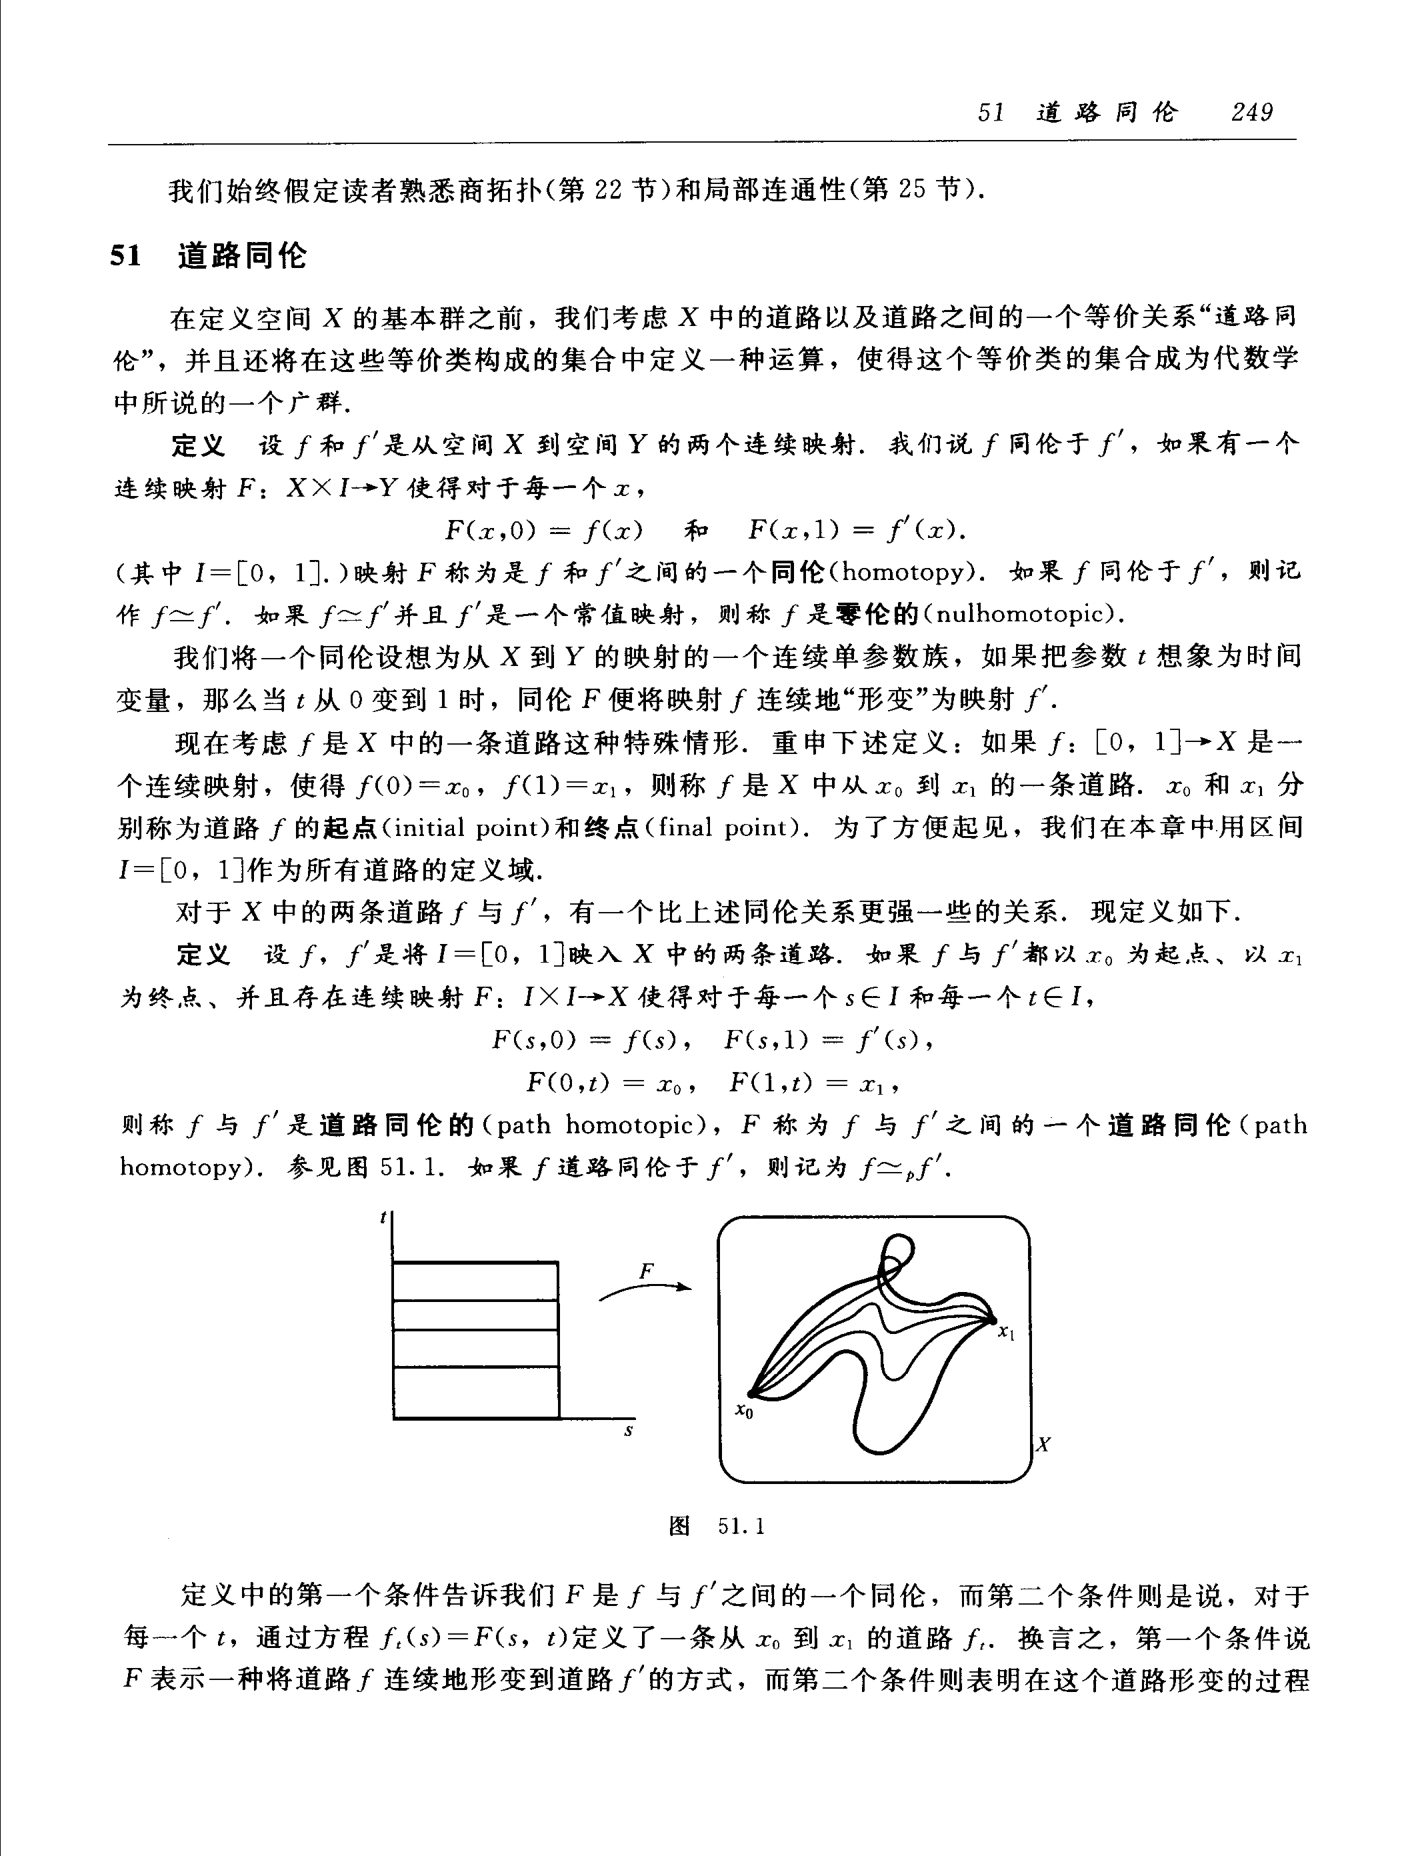
\includegraphics[width=0.7\textwidth]{image/fig-51-1.png}
\caption{道路同伦.}
\label{figure:ch09-fig-51-1}
\end{figure}

定义中的第一个条件告诉我们 $F$ 是 $f$ 与 $f'$ 之间的一个同伦, 而第二个条件则是说, 对于每一个 $t$, 通过方程 $f_t(s)=F(s,t)$ 定义了一条从 $x_0$ 到 $x_1$ 的道路 $f_t$. 换言之, 第一个条件说 $F$ 表示一种将道路 $f$ 连续地形变到道路 $f'$ 的方式, 而第二个条件则表明在这个道路形变的过程中端点保持不动.

\begin{lemma}
\label{lemma:ch09-sec51-51-1}
关系 $\simeq$ 和 $\simeq_p$ 都是等价关系. 如果 $f$ 是一条道路, 我们则记它的道路同伦等价类为 $[f]$.
\end{lemma}

\begin{proof}
我们来验证它们满足等价关系的条件.

对于给定的 $f$, 显然 $f\simeq f$, 因为映射 $F(x,t)=f(x)$ 就是所求的同伦. 如果 $f$ 是一条道路, $F$ 便是道路同伦.

如果 $f\simeq f'$, 我们证明 $f'\simeq f$. 设 $F$ 是 $f$ 与 $f'$ 之间的一个同伦, 则 $G(x,t)=F(x,1-t)$ 便是 $f'$ 与 $f$ 之间的一个同伦. 当 $F$ 是道路同伦时, $G$ 也是道路同伦.

设 $f\simeq f'$, $f'\simeq f''$. 我们证明 $f\simeq f''$. 设 $F$ 为 $f$ 与 $f'$ 之间的一个同伦, $F'$ 为 $f'$ 与 $f''$ 之间的一个同伦, 定义 $G\colon X\times I\to Y$ 如下:
\[
G(x,t)=
\begin{cases}
F(x,2t) & \text{当 }t\in\left[0,\frac{1}{2}\right],\\
F'(x,2t-1) & \text{当 }t\in\left[\frac{1}{2},1\right].
\end{cases}
\]
映射 $G$ 的定义是确切的, 因为当 $t=\frac{1}{2}$ 时, $F(x,2t)=f'(x)=F'(x,2t-1)$. 由于 $G$ 在 $X\times I$ 的两个闭子集 $X\times\left[0,\frac{1}{2}\right]$ 与 $X\times\left[\frac{1}{2},1\right]$ 上都是连续的, 根据黏结引理, $G$ 在 $X\times I$ 上也是连续的. 于是 $G$ 便是 $f$ 与 $f''$ 之间所求的同伦.

请自行验证当 $F$ 和 $F'$ 都是道路同伦时, $G$ 也是道路同伦. 参见图 \cref{figure:ch09-fig-51-2}.
\end{proof}

\par
\begin{figure}[htbp]
\centering
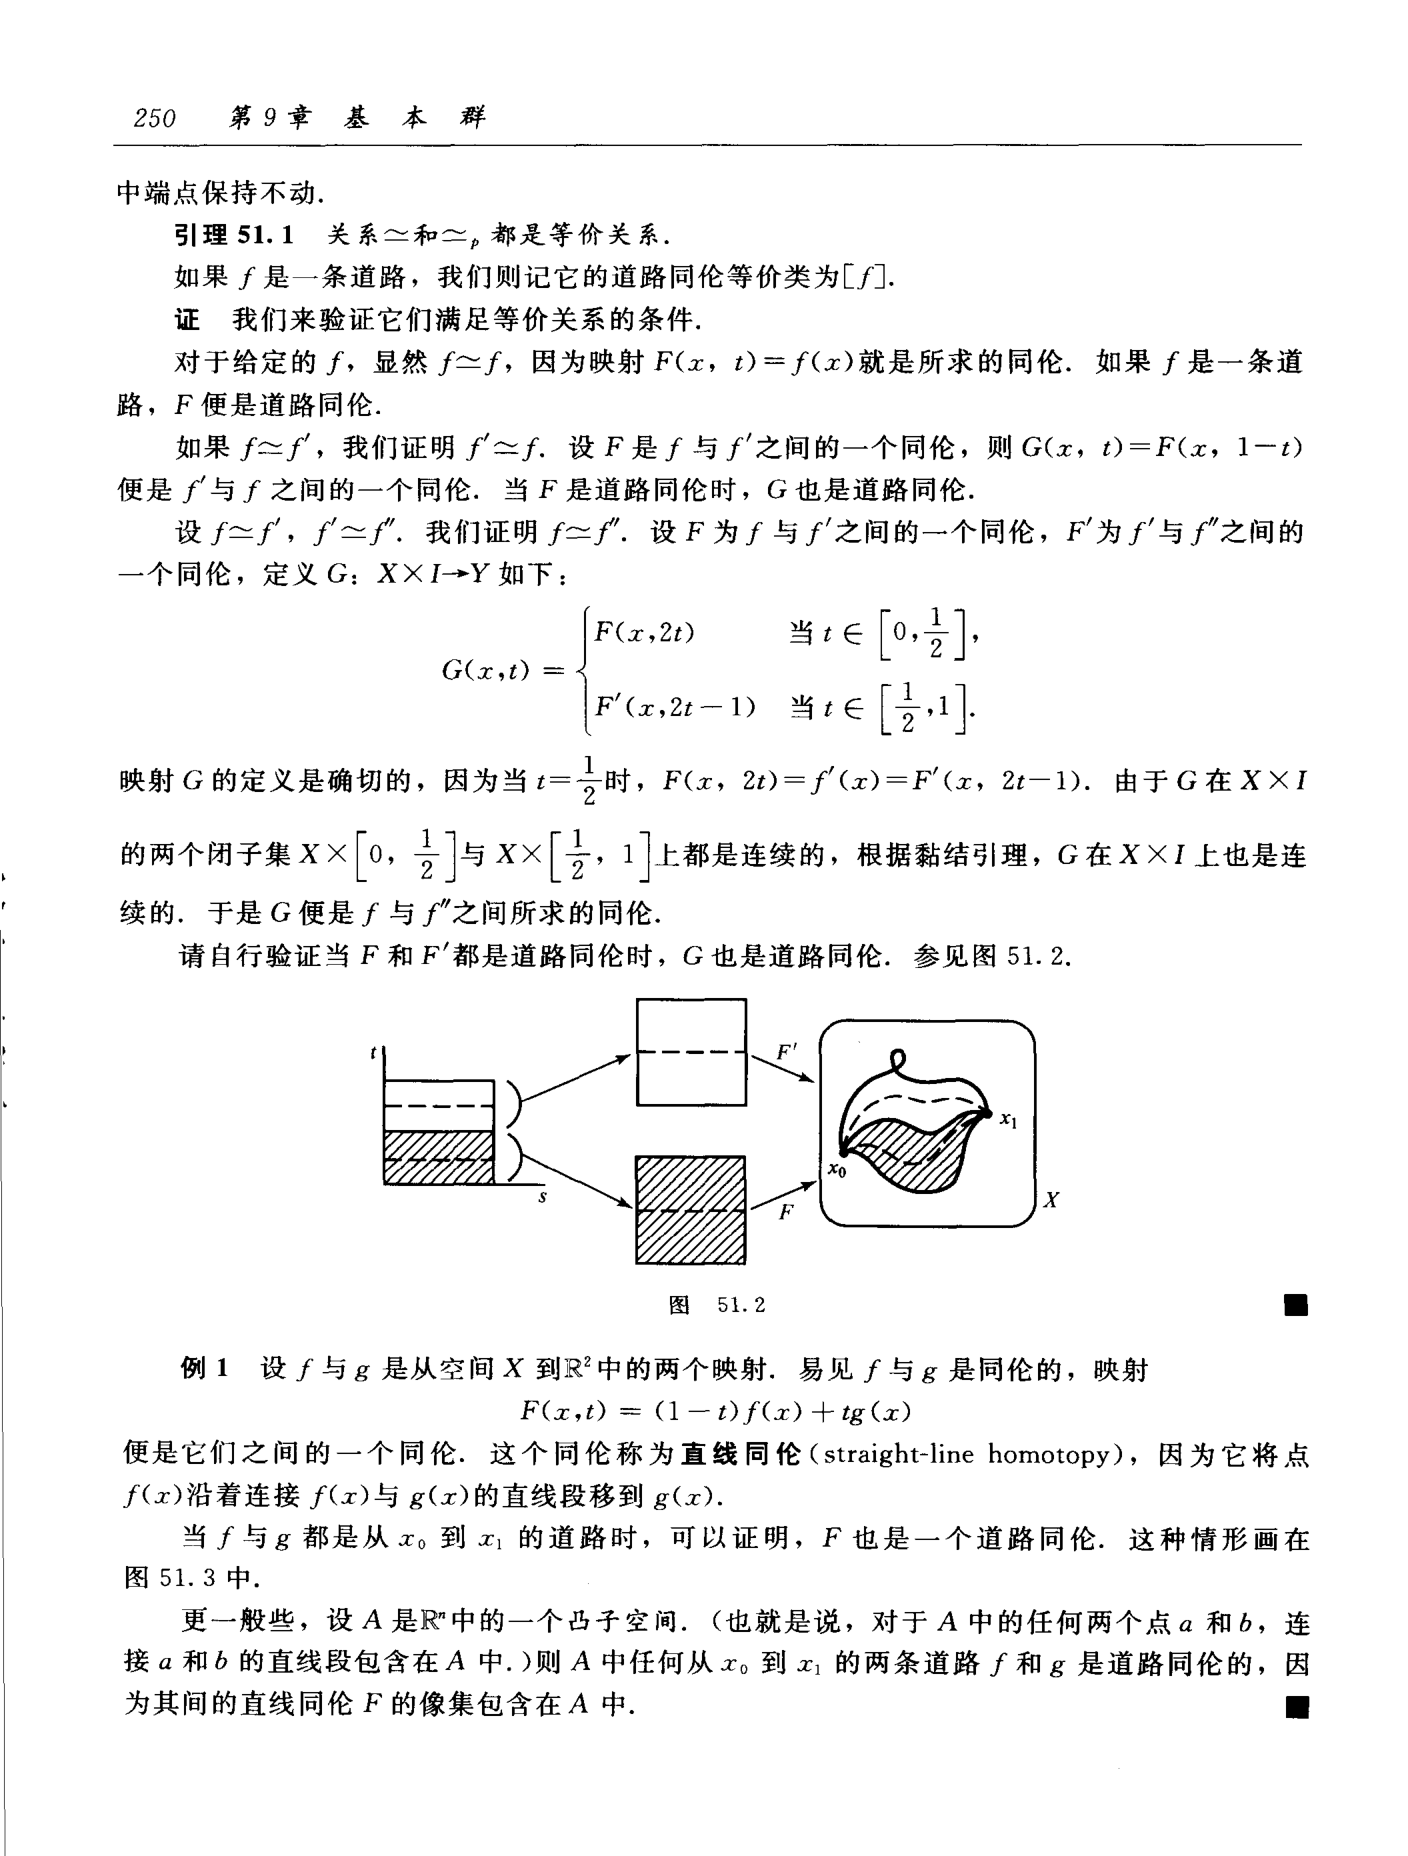
\includegraphics[width=0.7\textwidth]{image/fig-51-2.png}
\caption{同伦的黏结.}
\label{figure:ch09-fig-51-2}
\end{figure}

\begin{example}
\label{example:ch09-sec51-1}
设 $f$ 与 $g$ 是从空间 $X$ 到 $\mathbb{R}^{2}$ 中的两个映射. 易见 $f$ 与 $g$ 是同伦的, 映射
\[
F(x,t)=(1-t)f(x)+tg(x)
\]
便是它们之间的一个同伦. 这个同伦称为\textbf{直线同伦}(straight-line homotopy), 因为它将点 $f(x)$ 沿着连接 $f(x)$ 与 $g(x)$ 的直线段移到 $g(x)$.

当 $f$ 与 $g$ 都是从 $x_0$ 到 $x_1$ 的道路时, 可以证明, $F$ 也是一个道路同伦. 这种情形画在图 \cref{figure:ch09-fig-51-3} 中.

更一般地, 设 $A$ 是 $\mathbb{R}^{n}$ 中的一个凸子空间. (也就是说, 对于 $A$ 中的任何两个点 $a$ 和 $b$, 连接 $a$ 和 $b$ 的直线段包含在 $A$ 中.) 则 $A$ 中任何从 $x_0$ 到 $x_1$ 的两条道路 $f$ 和 $g$ 是道路同伦的, 因为其间的直线同伦 $F$ 的像集包含在 $A$ 中.
\end{example}

\par
\begin{figure}[htbp]
\centering
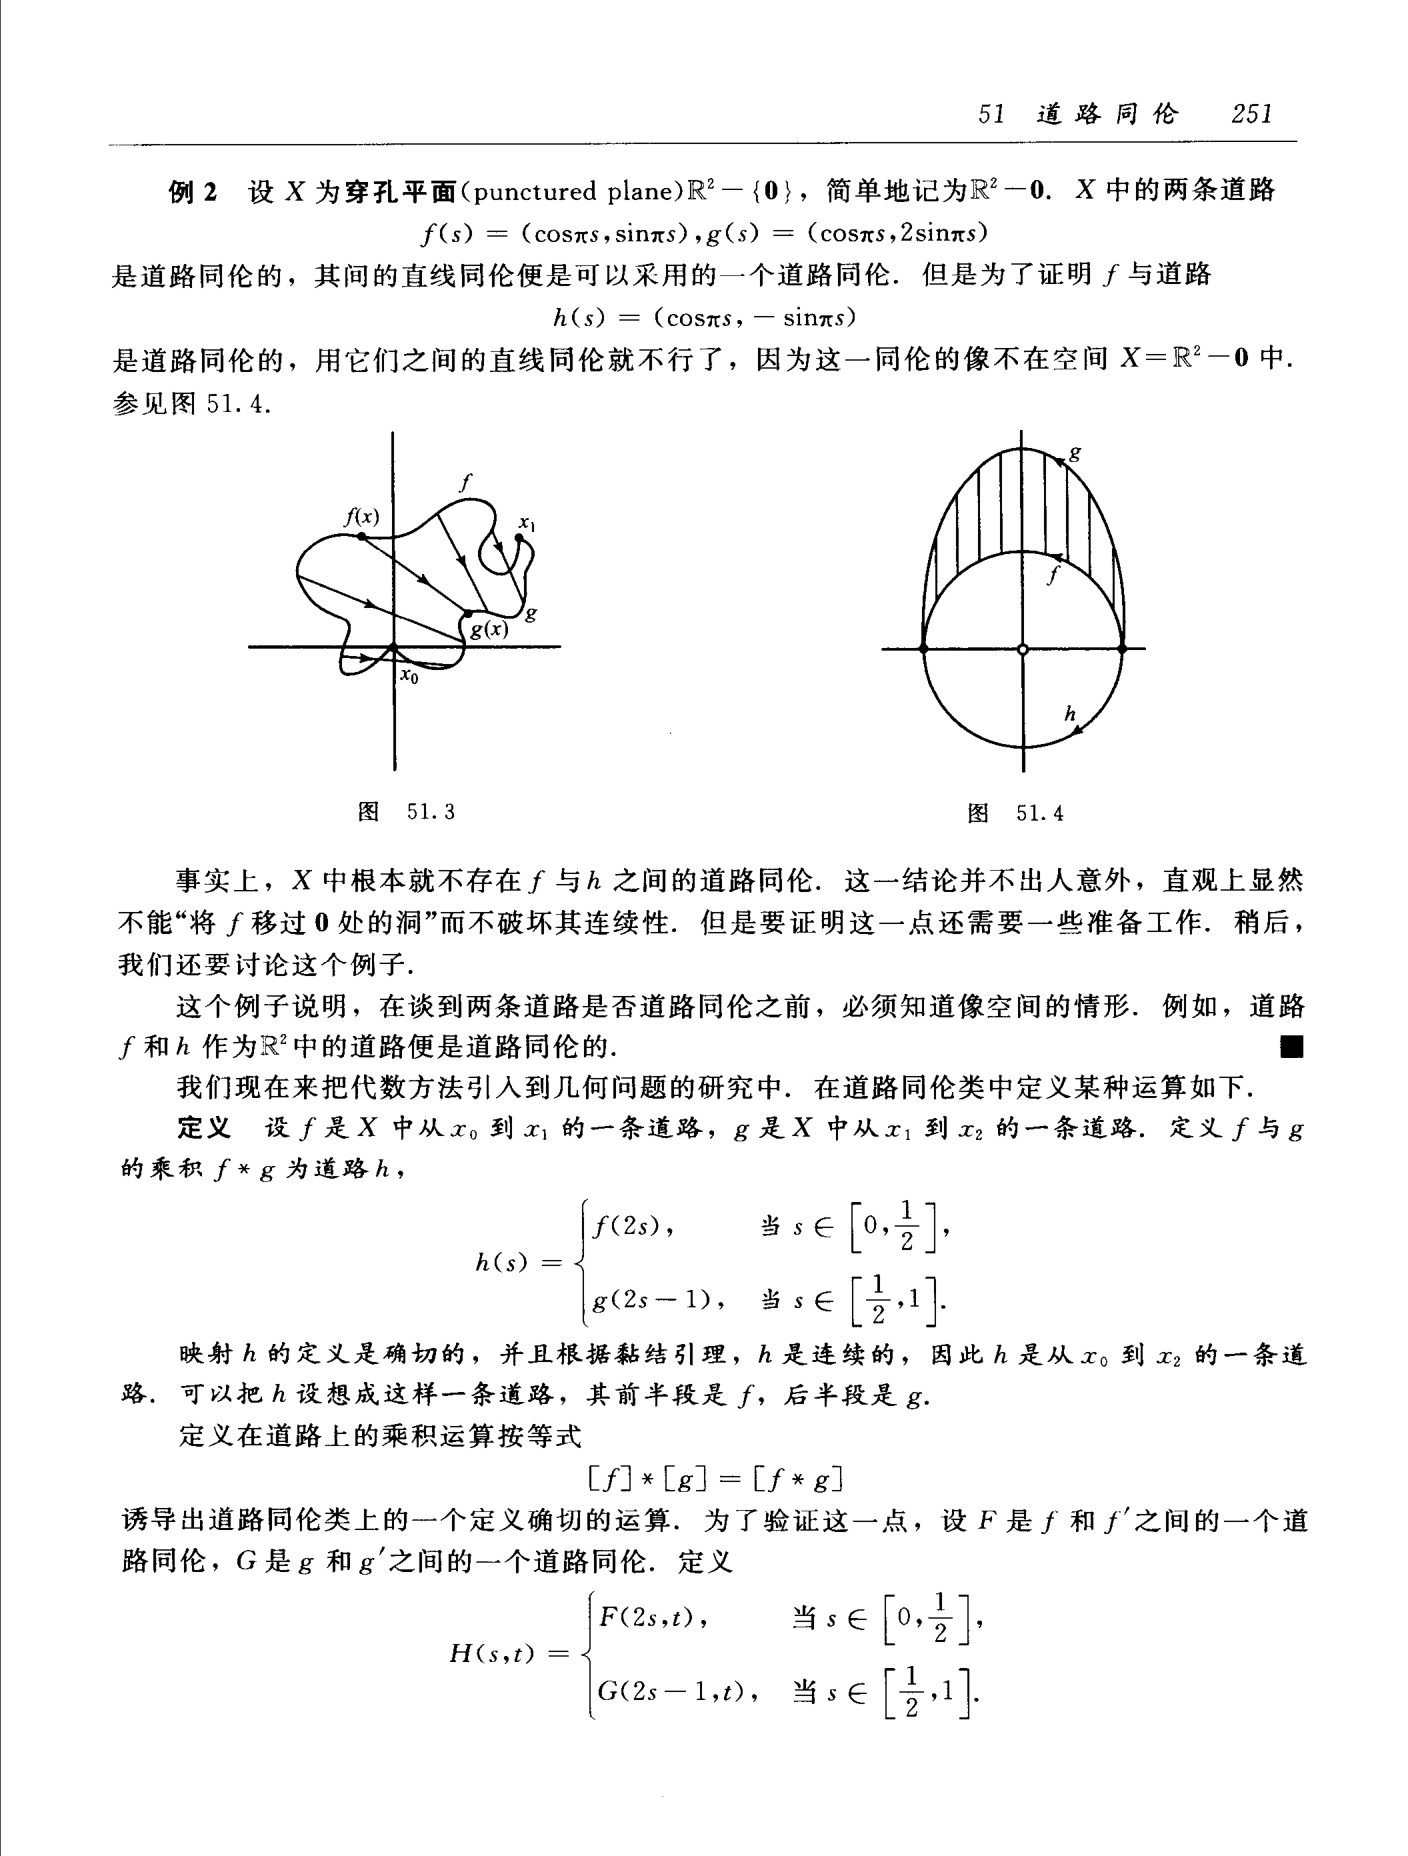
\includegraphics[width=0.5\textwidth]{image/fig-51-3.png}
\caption{直线同伦.}
\label{figure:ch09-fig-51-3}
\end{figure}

\begin{example}
\label{example:ch09-sec51-2}
设 $X$ 为\textbf{穿孔平面}(punctured plane) $\mathbb{R}^{2}-\{\boldsymbol{0}\}$, 简单地记为 $\mathbb{R}^{2}-\boldsymbol{0}$. $X$ 中的两条道路
\[
f(s)=(\cos\pi s,\sin\pi s),\quad g(s)=(\cos\pi s,2\sin\pi s)
\]
是道路同伦的, 其间的直线同伦便是可以采用的一个道路同伦. 但是为了证明 $f$ 与道路
\[
h(s)=(\cos\pi s,-\sin\pi s)
\]
是道路同伦的, 用它们之间的直线同伦就不行了, 因为这一同伦的像不在空间 $X=\mathbb{R}^{2}-\boldsymbol{0}$ 中. 参见图 \cref{figure:ch09-fig-51-4}.

事实上, $X$ 中根本就不存在 $f$ 与 $h$ 之间的道路同伦. 这一结论并不出人意外, 直观上显然不能"将 $f$ 移过 $\boldsymbol{0}$ 处的洞"而不破坏其连续性. 但是要证明这一点还需要一些准备工作. 稍后, 我们还要讨论这个例子.

这个例子说明, 在谈到两条道路是否道路同伦之前, 必须知道像空间的情形. 例如, 道路 $f$ 和 $h$ 作为 $\mathbb{R}^{2}$ 中的道路便是道路同伦的.
\end{example}

\par
\begin{figure}[htbp]
\centering
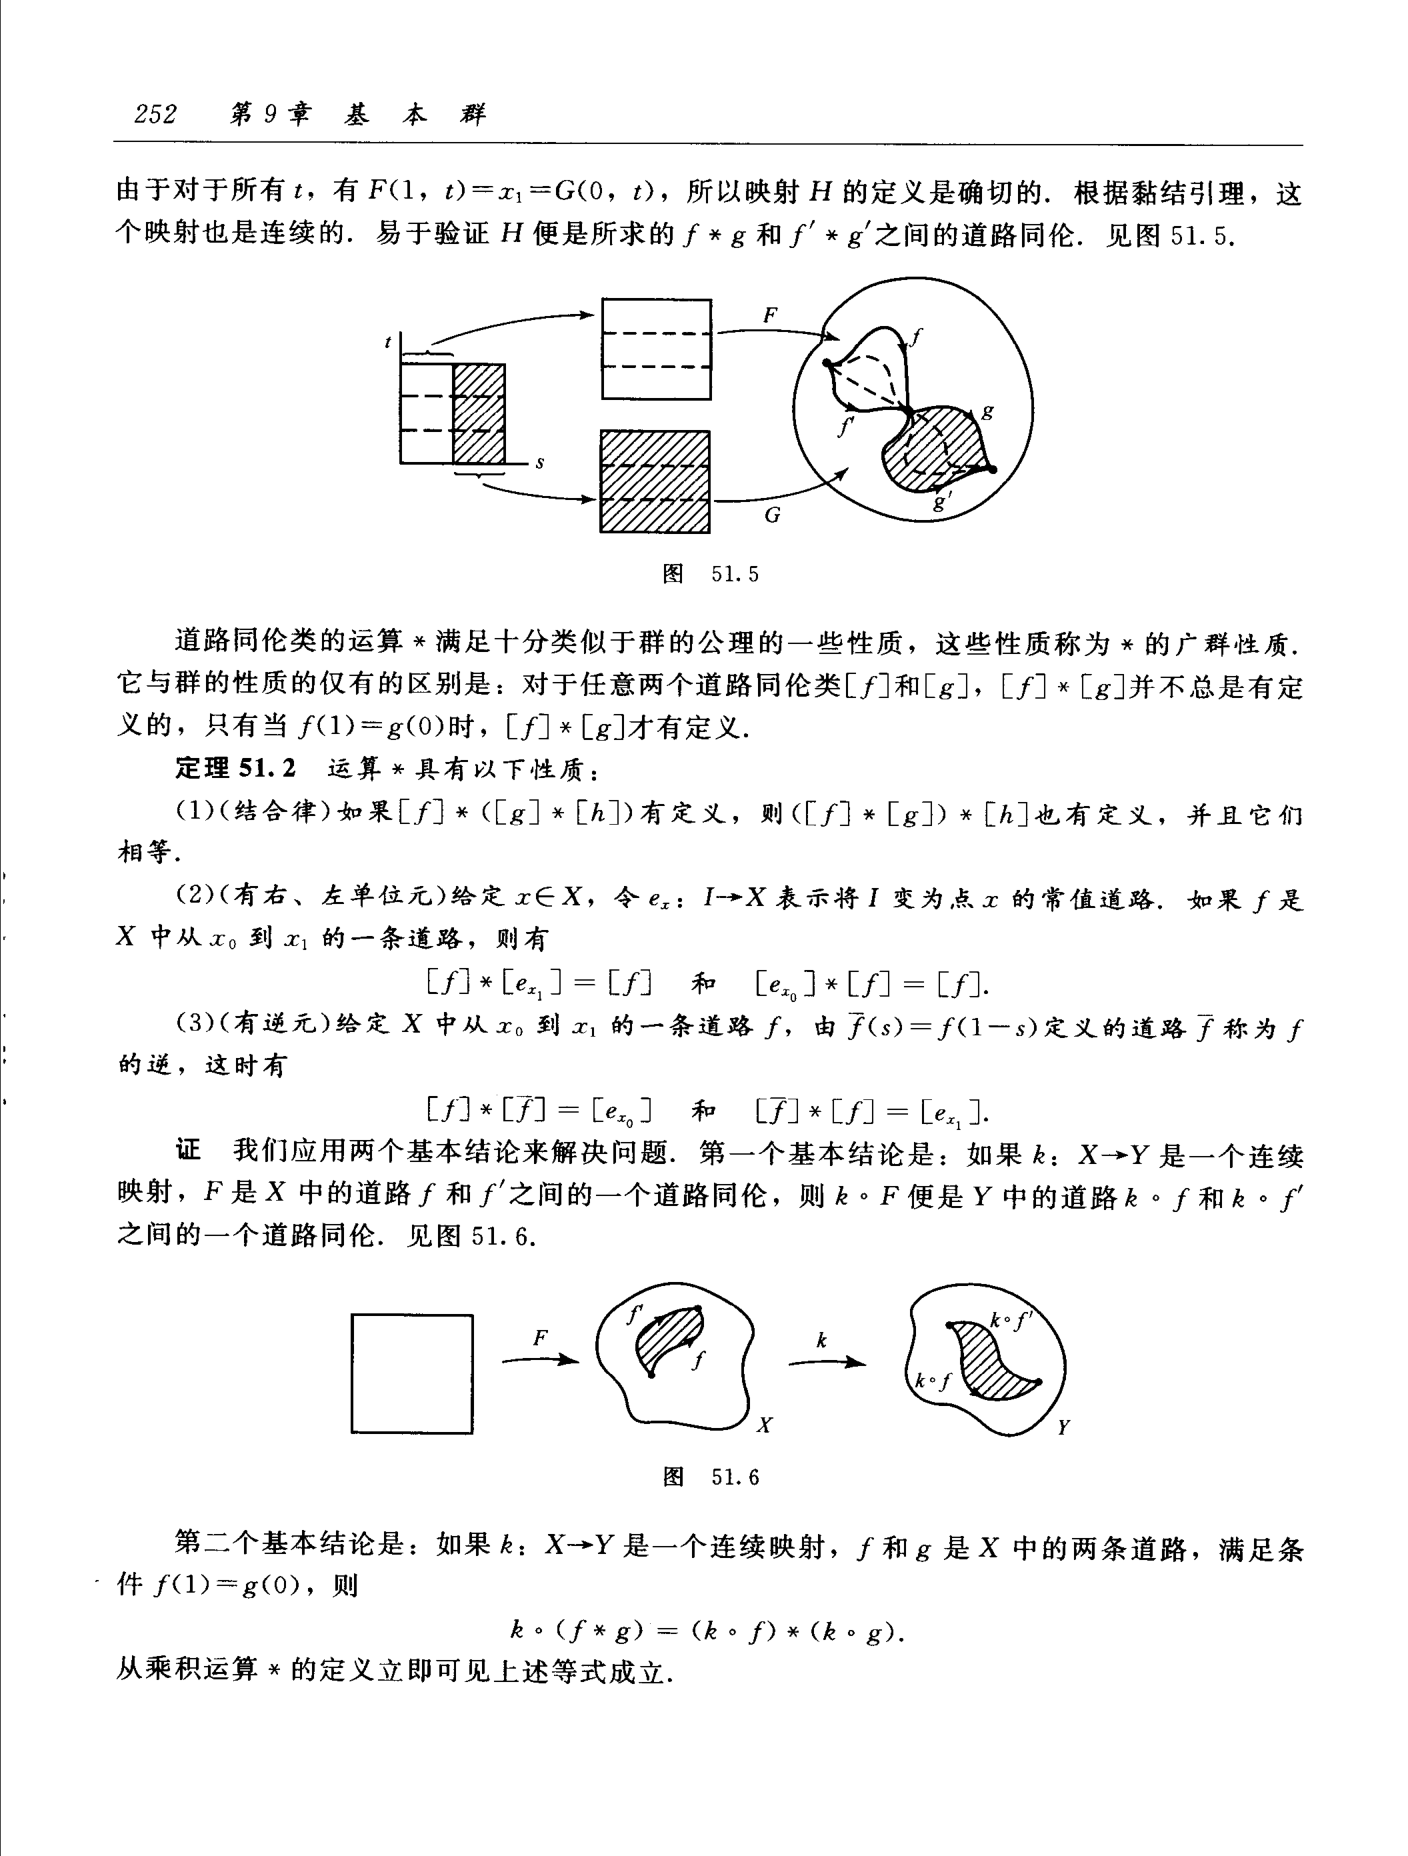
\includegraphics[width=0.6\textwidth]{image/fig-51-4.png}
\caption{穿孔平面中的道路.}
\label{figure:ch09-fig-51-4}
\end{figure}

我们现在来把代数方法引入到几何问题的研究中. 在道路同伦类中定义某种运算如下.

\begin{definition}[道路的乘积]
\label{definition:ch09-sec51-product}
设 $f$ 是 $X$ 中从 $x_0$ 到 $x_1$ 的一条道路, $g$ 是 $X$ 中从 $x_1$ 到 $x_2$ 的一条道路. 定义 $f$ 与 $g$ 的\textbf{乘积} $f*g$ 为道路 $h$,
\[
h(s)=
\begin{cases}
f(2s), & \text{当 }s\in\left[0,\frac{1}{2}\right],\\
g(2s-1), & \text{当 }s\in\left[\frac{1}{2},1\right].
\end{cases}
\]
\end{definition}

映射 $h$ 的定义是确切的, 并且根据黏结引理, $h$ 是连续的, 因此 $h$ 是从 $x_0$ 到 $x_2$ 的一条道路. 可以把 $h$ 设想成这样一条道路, 其前半段是 $f$, 后半段是 $g$.

定义在道路上的乘积运算按等式
\[
[f]*[g]=[f*g]
\]
诱导出道路同伦类上的一个定义确切的运算. 为了验证这一点, 设 $F$ 是 $f$ 和 $f'$ 之间的一个道路同伦, $G$ 是 $g$ 和 $g'$ 之间的一个道路同伦. 定义
\[
H(s,t)=
\begin{cases}
F(2s,t), & \text{当 }s\in\left[0,\frac{1}{2}\right],\\
G(2s-1,t), & \text{当 }s\in\left[\frac{1}{2},1\right].
\end{cases}
\]
由于对于所有 $t$, 有 $F(1,t)=x_1=G(0,t)$, 所以映射 $H$ 的定义是确切的. 根据黏结引理, 这个映射也是连续的. 易于验证 $H$ 便是所求的 $f*g$ 和 $f'*g'$ 之间的道路同伦. 见图 \cref{figure:ch09-fig-51-5}.

\par
\begin{figure}[htbp]
\centering
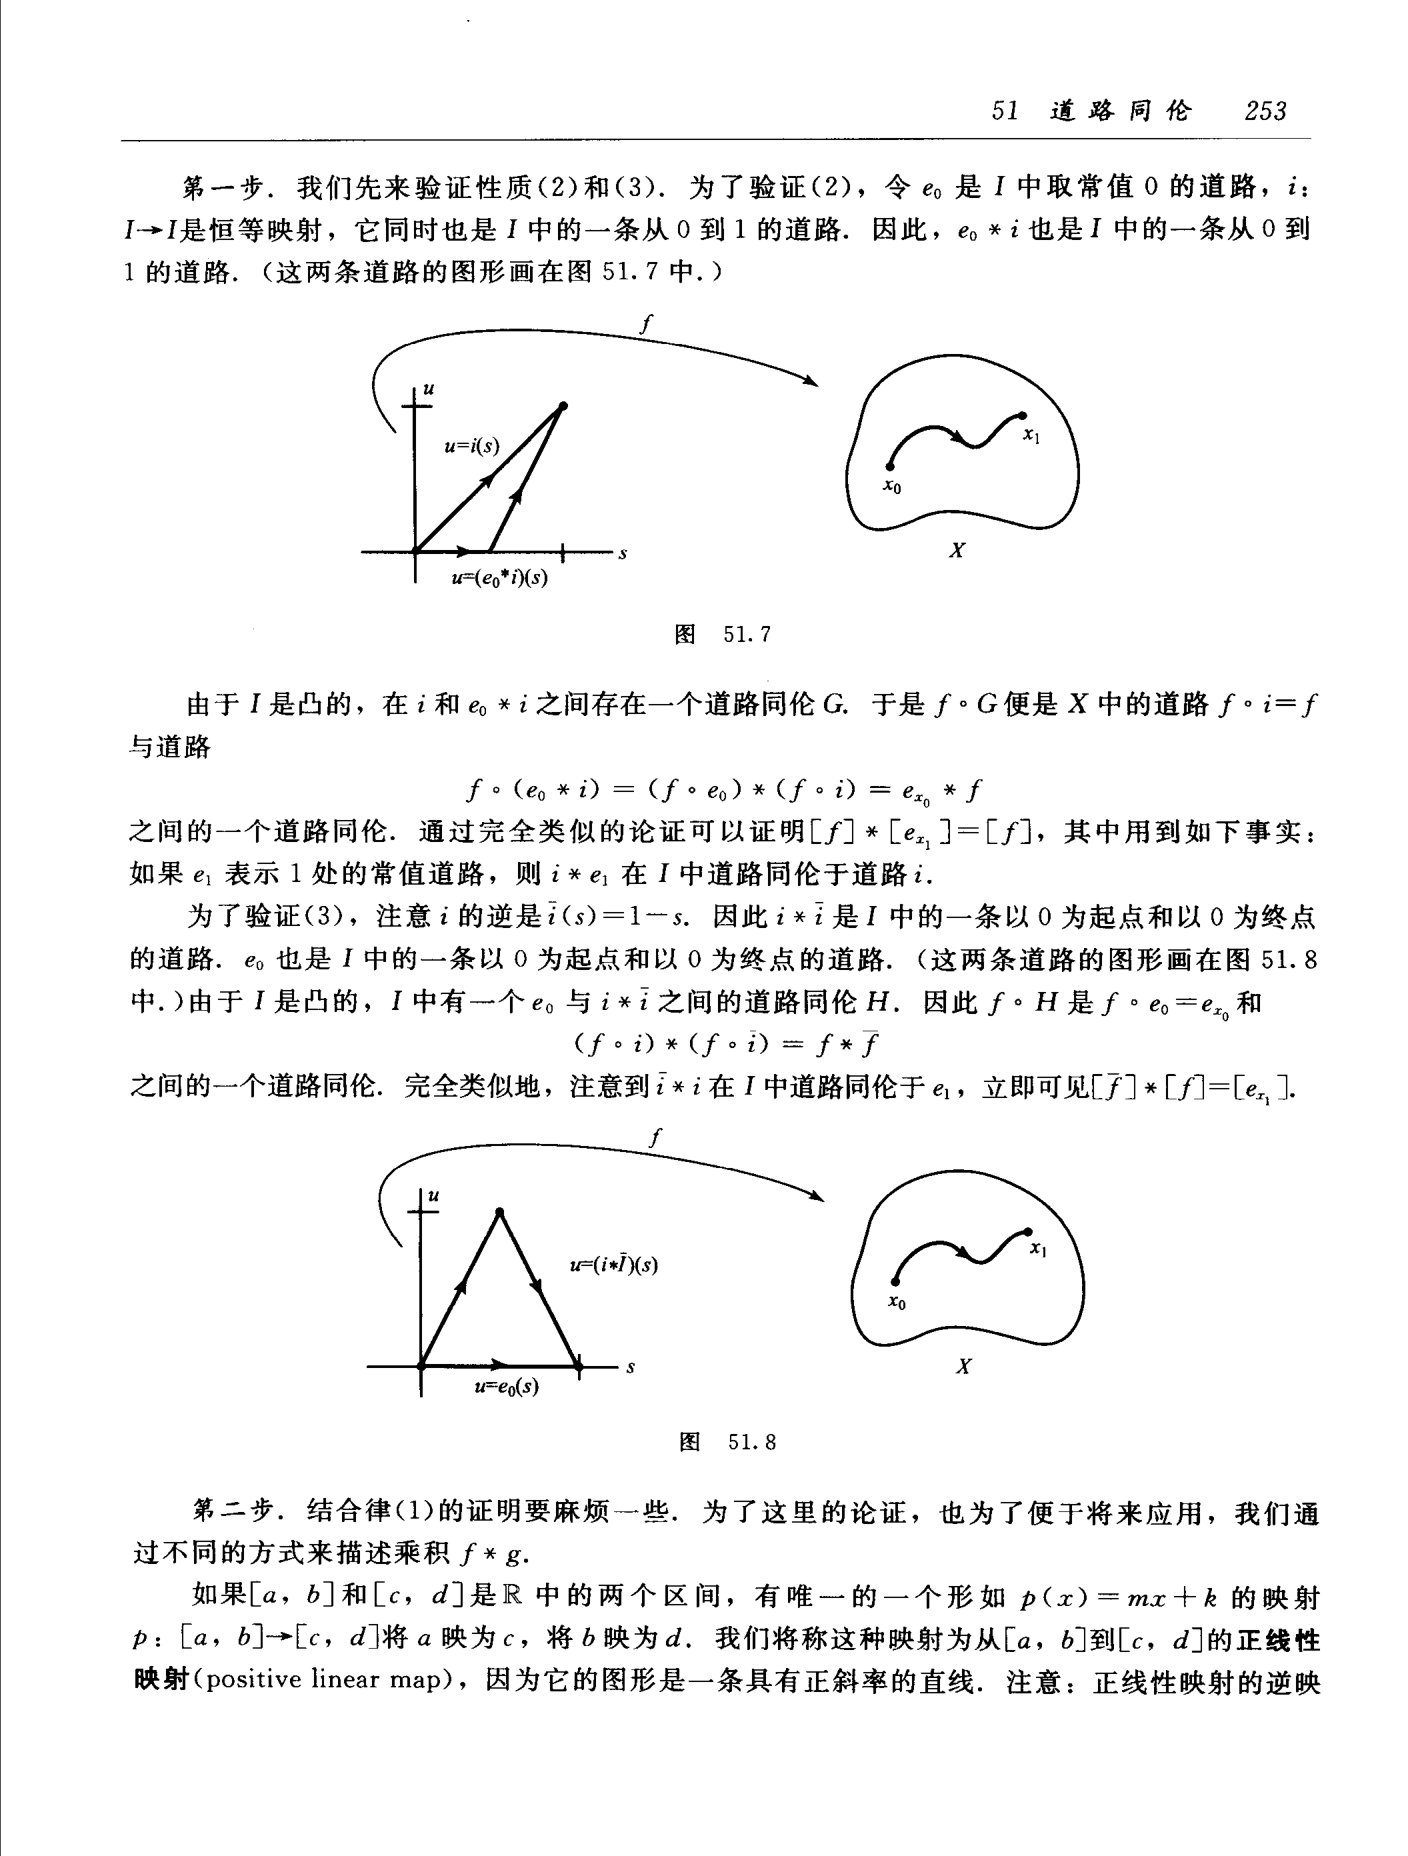
\includegraphics[width=0.7\textwidth]{image/fig-51-5.png}
\caption{道路乘积的同伦.}
\label{figure:ch09-fig-51-5}
\end{figure}

道路同伦类的运算 $*$ 满足十分类似于群的公理的一些性质, 这些性质称为 $*$ 的\textbf{广群性质}. 它与群的性质的仅有的区别是: 对于任意两个道路同伦类 $[f]$ 和 $[g]$, $[f]*[g]$ 并不总是有定义的, 只有当 $f(1)=g(0)$ 时, $[f]*[g]$ 才有定义.

\begin{theorem}
\label{theorem:ch09-sec51-51-2}
运算 $*$ 具有以下性质:
\begin{enumerate}
\item (\textbf{结合律}) 如果 $[f]*([g]*[h])$ 有定义, 则 $([f]*[g])*[h]$ 也有定义, 并且它们相等.
\item (\textbf{有右、左单位元}) 给定 $x\in X$, 令 $e_x\colon I\to X$ 表示将 $I$ 变为点 $x$ 的常值道路. 如果 $f$ 是 $X$ 中从 $x_0$ 到 $x_1$ 的一条道路, 则有
\[
[f]*[e_{x_{1}}]=[f]\quad\text{和}\quad[e_{x_{0}}]*[f]=[f].
\]
\item (\textbf{有逆元}) 给定 $X$ 中从 $x_0$ 到 $x_1$ 的一条道路 $f$, 由 $\bar{f}(s)=f(1-s)$ 定义的道路 $\bar{f}$ 称为 $f$ 的\textbf{逆}, 这时有
\[
[f]*[\bar{f}]=[e_{x_{0}}]\quad\text{和}\quad[\bar{f}]*[f]=[e_{x_{1}}].
\]
\end{enumerate}
\end{theorem}

\par
\begin{figure}[htbp]
\centering
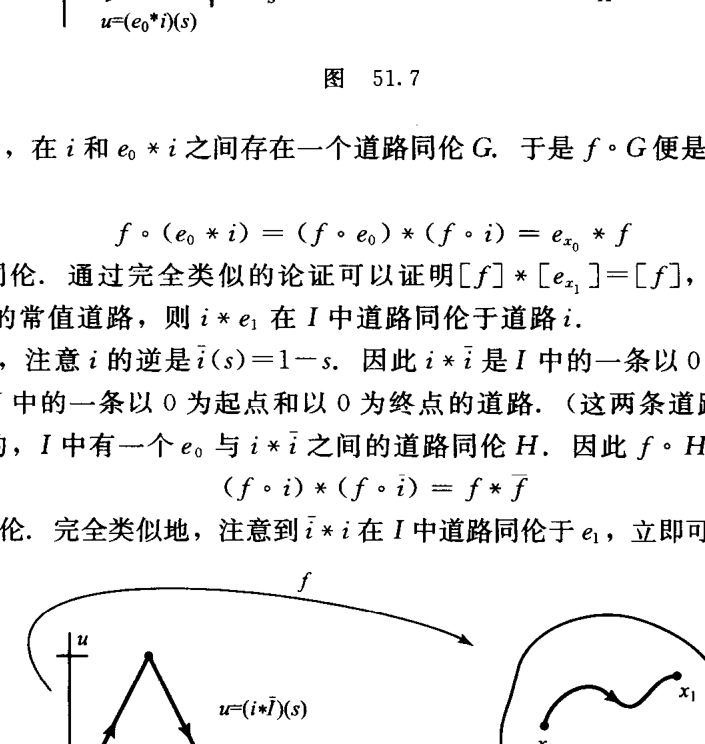
\includegraphics[width=0.7\textwidth]{image/fig-51-6.png}
\caption{连续映射保持道路同伦.}
\label{figure:ch09-fig-51-6}
\end{figure}

\par
\begin{figure}[htbp]
\centering
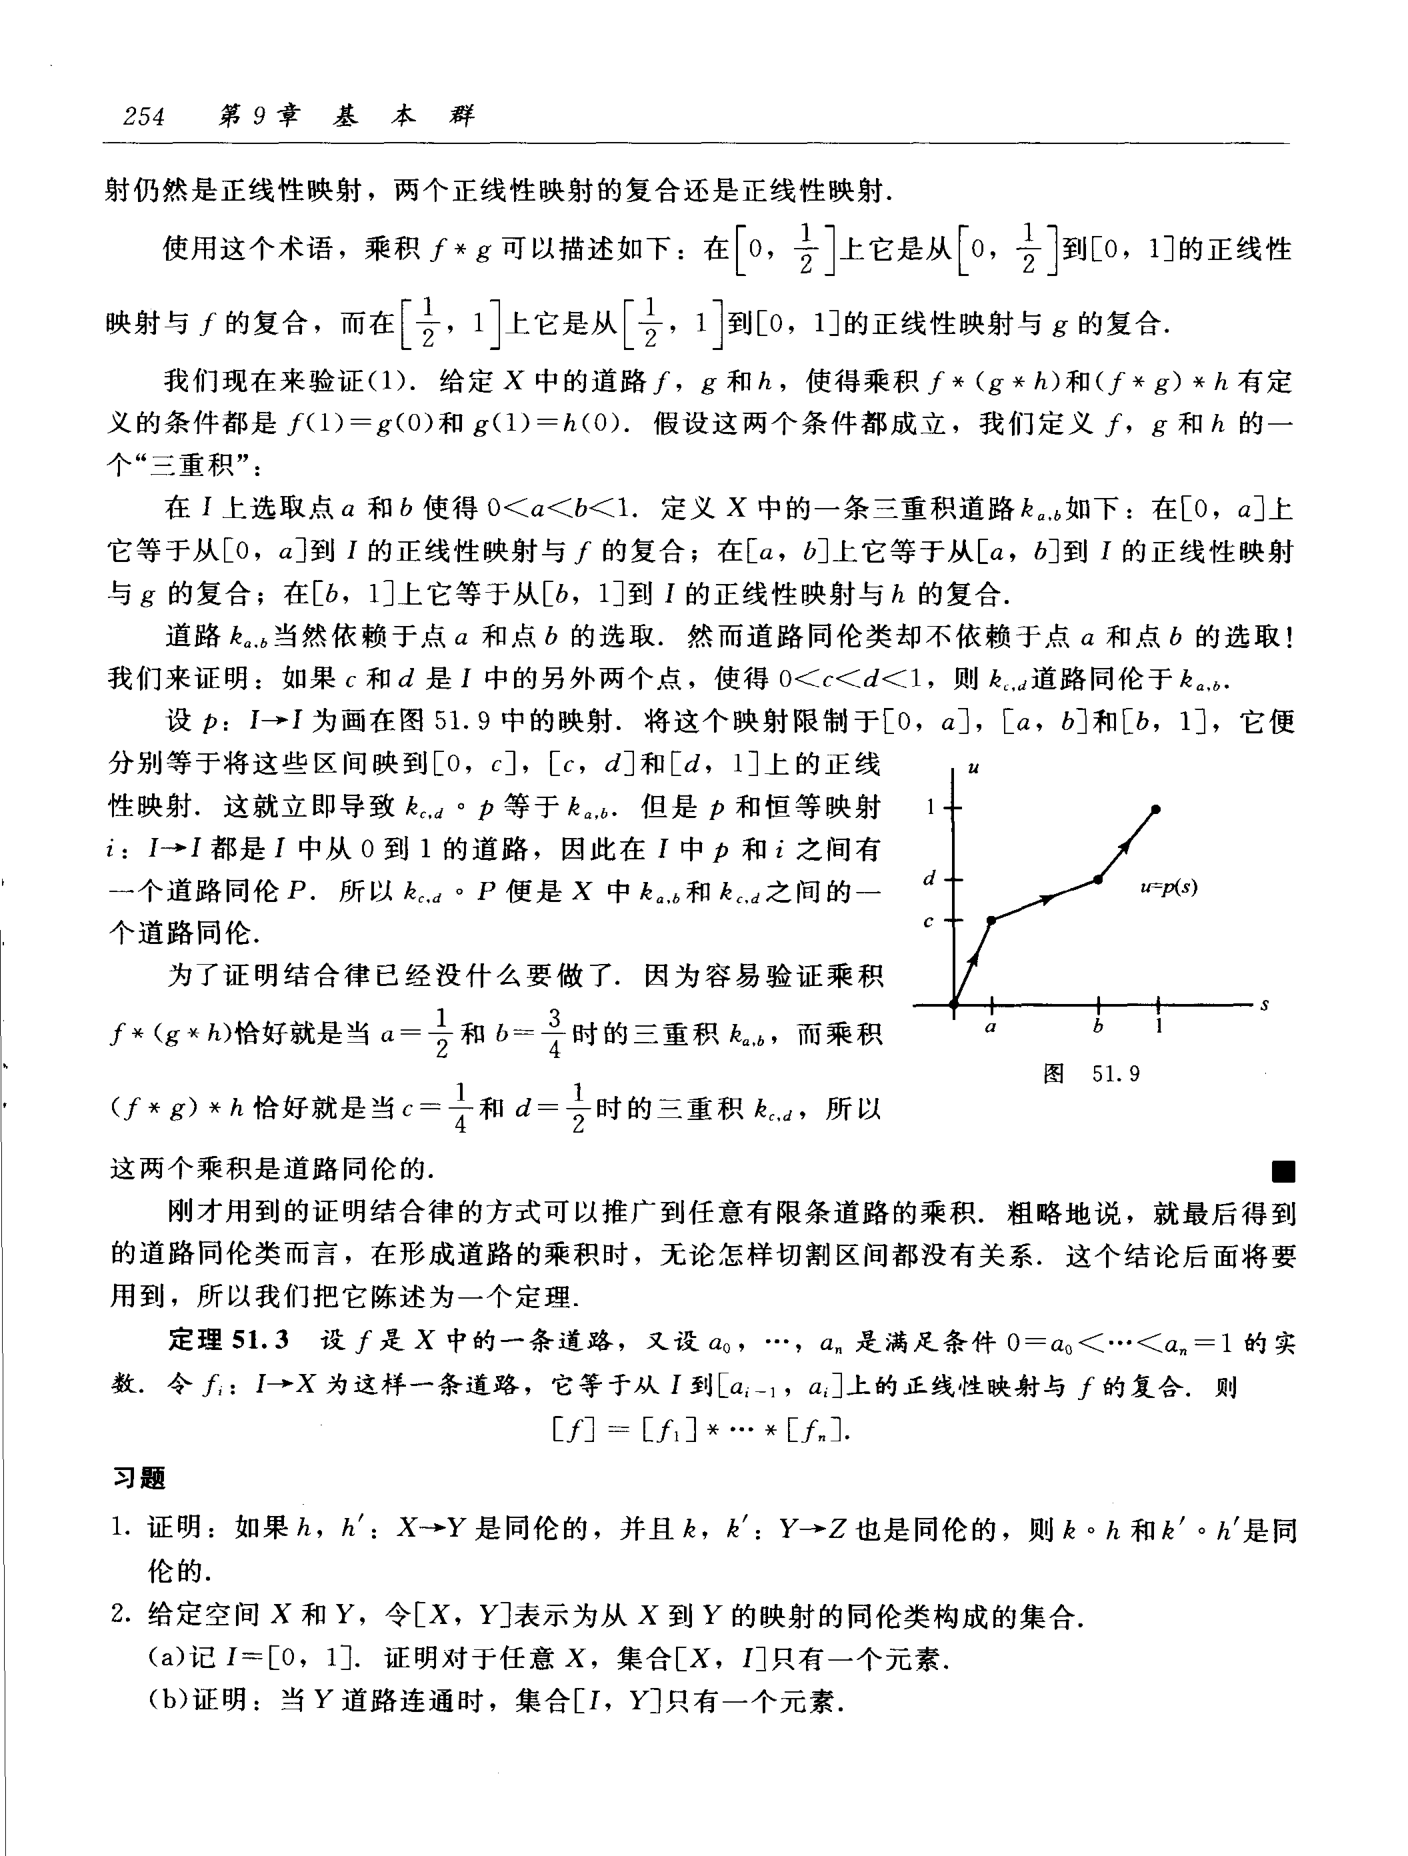
\includegraphics[width=0.6\textwidth]{image/fig-51-7.png}
\caption{$e_0*i$ 与 $i$ 的同伦.}
\label{figure:ch09-fig-51-7}
\end{figure}

\par
\begin{figure}[htbp]
\centering
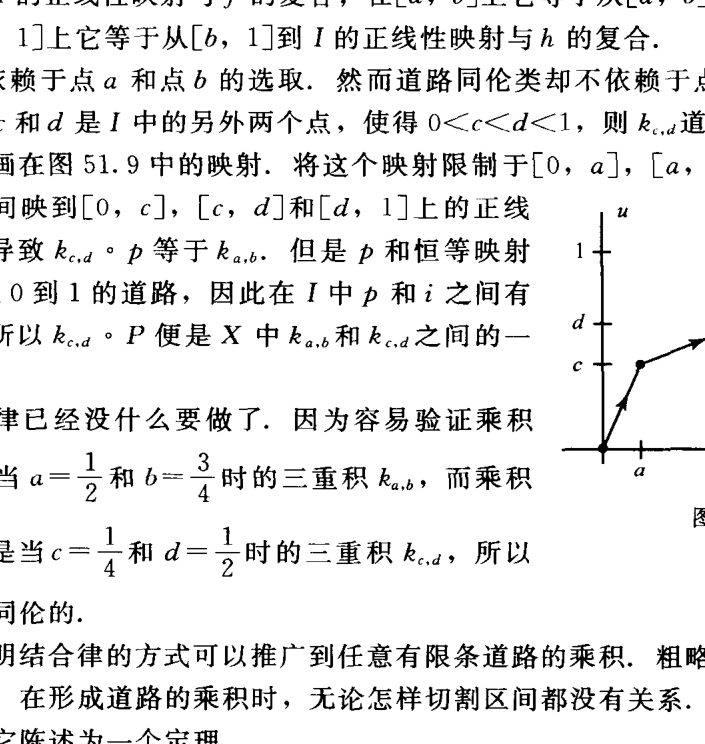
\includegraphics[width=0.6\textwidth]{image/fig-51-8.png}
\caption{$i*\bar{i}$ 与 $e_0$ 的同伦.}
\label{figure:ch09-fig-51-8}
\end{figure}

\par
\begin{figure}[htbp]
\centering
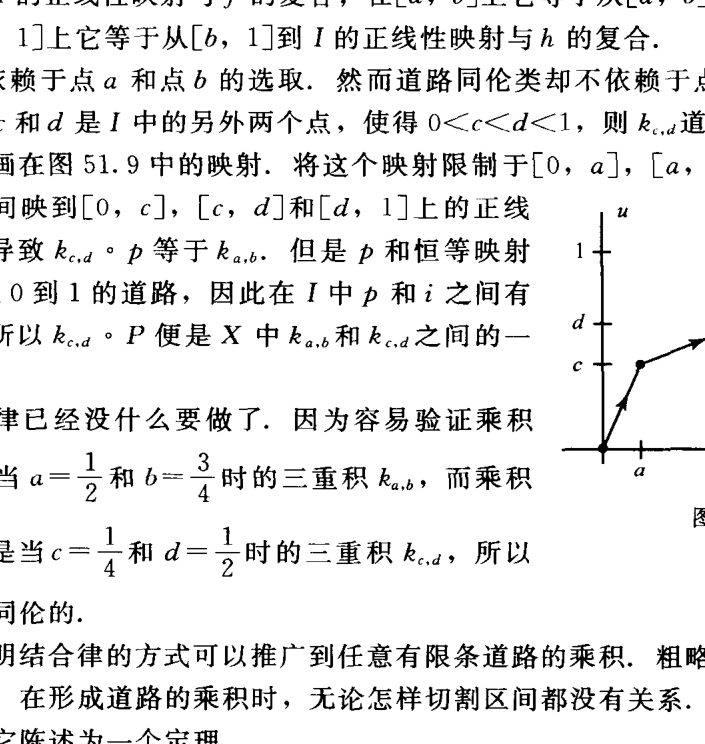
\includegraphics[width=0.5\textwidth]{image/fig-51-9.png}
\caption{正线性映射 $p$.}
\label{figure:ch09-fig-51-9}
\end{figure}

\begin{proof}
我们应用两个基本结论来解决问题. 第一个基本结论是: 如果 $k\colon X\to Y$ 是一个连续映射, $F$ 是 $X$ 中的道路 $f$ 和 $f'$ 之间的一个道路同伦, 则 $k\circ F$ 便是 $Y$ 中的道路 $k\circ f$ 和 $k\circ f'$ 之间的一个道路同伦. 见图 \cref{figure:ch09-fig-51-6}.


第二个基本结论是: 如果 $k\colon X\to Y$ 是一个连续映射, $f$ 和 $g$ 是 $X$ 中的两条道路, 满足条件 $f(1)=g(0)$, 则
\[
k\circ(f*g)=(k\circ f)*(k\circ g).
\]
从乘积运算 $*$ 的定义立即可见上述等式成立.

\textbf{第一步}. 我们先来验证性质 (2) 和 (3). 为了验证 (2), 令 $e_0$ 是 $I$ 中取常值 $0$ 的道路, $i\colon I\to I$ 是恒等映射, 它同时也是 $I$ 中的一条从 $0$ 到 $1$ 的道路. 因此, $e_0*i$ 也是 $I$ 中的一条从 $0$ 到 $1$ 的道路. (这两条道路的图形画在图 \cref{figure:ch09-fig-51-7} 中.)


由于 $I$ 是凸的, 在 $i$ 和 $e_0*i$ 之间存在一个道路同伦 $G$. 于是 $f\circ G$ 便是 $X$ 中的道路 $f\circ i=f$ 与道路
\[
f\circ(e_{0}*i)=(f\circ e_{0})*(f\circ i)=e_{x_{0}}*f
\]
之间的一个道路同伦. 通过完全类似的论证可以证明 $[f]*[e_{x_1}]=[f]$, 其中用到如下事实: 如果 $e_1$ 表示 $1$ 处的常值道路, 则 $i*e_1$ 在 $I$ 中道路同伦于道路 $i$.

为了验证 (3), 注意 $i$ 的逆是 $\bar{i}(s)=1-s$. 因此 $i*\bar{i}$ 是 $I$ 中的一条以 $0$ 为起点和以 $0$ 为终点的道路. $e_0$ 也是 $I$ 中的一条以 $0$ 为起点和以 $0$ 为终点的道路. (这两条道路的图形画在图 \cref{figure:ch09-fig-51-8} 中.) 由于 $I$ 是凸的, $I$ 中有一个 $e_0$ 与 $i*\bar{i}$ 之间的道路同伦 $H$. 因此 $f\circ H$ 是 $f\circ e_0=e_{x_0}$ 和
\[
(f\circ i)*(f\circ\bar{i})=f*\bar{f}
\]
之间的一个道路同伦. 完全类似地, 注意到 $\bar{i}*i$ 在 $I$ 中道路同伦于 $e_1$, 立即可见 $[\bar{f}]*[f]=[e_{x_1}]$.


\textbf{第二步}. 结合律 (1) 的证明要麻烦一些. 为了这里的论证, 也为了便于将来应用, 我们通过不同的方式来描述乘积 $f*g$.

如果 $[a,b]$ 和 $[c,d]$ 是 $\mathbb{R}$ 中的两个区间, 有唯一的一个形如 $p(x)=mx+k$ 的映射 $p\colon[a,b]\to[c,d]$ 将 $a$ 映为 $c$, 将 $b$ 映为 $d$. 我们将称这种映射为从 $[a,b]$ 到 $[c,d]$ 的\textbf{正线性映射}(positive linear map), 因为它的图形是一条具有正斜率的直线. 注意: 正线性映射的逆映射仍然是正线性映射, 两个正线性映射的复合还是正线性映射.

使用这个术语, 乘积 $f*g$ 可以描述如下: 在 $\left[0,\frac{1}{2}\right]$ 上它是从 $\left[0,\frac{1}{2}\right]$ 到 $[0,1]$ 的正线性映射与 $f$ 的复合, 而在 $\left[\frac{1}{2},1\right]$ 上它是从 $\left[\frac{1}{2},1\right]$ 到 $[0,1]$ 的正线性映射与 $g$ 的复合.

我们现在来验证 (1). 给定 $X$ 中的道路 $f$, $g$ 和 $h$, 使得乘积 $f*(g*h)$ 和 $(f*g)*h$ 有定义的条件都是 $f(1)=g(0)$ 和 $g(1)=h(0)$. 假设这两个条件都成立, 我们定义 $f$, $g$ 和 $h$ 的一个"三重积":

在 $I$ 上选取点 $a$ 和 $b$ 使得 $0<a<b<1$. 定义 $X$ 中的一条三重积道路 $k_{a,b}$ 如下: 在 $[0,a]$ 上它等于从 $[0,a]$ 到 $I$ 的正线性映射与 $f$ 的复合; 在 $[a,b]$ 上它等于从 $[a,b]$ 到 $I$ 的正线性映射与 $g$ 的复合; 在 $[b,1]$ 上它等于从 $[b,1]$ 到 $I$ 的正线性映射与 $h$ 的复合.

道路 $k_{a,b}$ 当然依赖于点 $a$ 和点 $b$ 的选取. 然而道路同伦类却不依赖于点 $a$ 和点 $b$ 的选取! 我们来证明: 如果 $c$ 和 $d$ 是 $I$ 中的另外两个点, 使得 $0<c<d<1$, 则 $k_{c,d}$ 道路同伦于 $k_{a,b}$.

设 $p\colon I\to I$ 为画在图 \cref{figure:ch09-fig-51-9} 中的映射. 将这个映射限制于 $[0,a]$, $[a,b]$ 和 $[b,1]$, 它便分别等于将这些区间映到 $[0,c]$, $[c,d]$ 和 $[d,1]$ 上的正线性映射. 这就立即导致 $k_{c,d}\circ p$ 等于 $k_{a,b}$. 但是 $p$ 和恒等映射 $i\colon I\to I$ 都是 $I$ 中从 $0$ 到 $1$ 的道路, 因此在 $I$ 中 $p$ 和 $i$ 之间有一个道路同伦 $P$. 所以 $k_{c,d}\circ P$ 便是 $X$ 中 $k_{a,b}$ 和 $k_{c,d}$ 之间的一个道路同伦.


为了证明结合律已经没什么要做了. 因为容易验证乘积 $f*(g*h)$ 恰好就是当 $a=\frac{1}{2}$ 和 $b=\frac{3}{4}$ 时的三重积 $k_{a,b}$, 而乘积 $(f*g)*h$ 恰好就是当 $c=\frac{1}{4}$ 和 $d=\frac{1}{2}$ 时的三重积 $k_{c,d}$, 所以这两个乘积是道路同伦的.
\end{proof}

刚才用到的证明结合律的方式可以推广到任意有限条道路的乘积. 粗略地说, 就最后得到的道路同伦类而言, 在形成道路的乘积时, 无论怎样切割区间都没有关系. 这个结论后面将要用到, 所以我们把它陈述为一个定理.

\begin{theorem}
\label{theorem:ch09-sec51-51-3}
设 $f$ 是 $X$ 中的一条道路, 又设 $a_0,\cdots,a_n$ 是满足条件 $0=a_0<\cdots<a_n=1$ 的实数. 令 $f_i\colon I\to X$ 为这样一条道路, 它等于从 $I$ 到 $[a_{i-1},a_i]$ 上的正线性映射与 $f$ 的复合. 则
\[
[f]=[f_{1}]*\cdots*[f_{n}].
\]
\end{theorem}

\subsection*{习题}

\begin{exercise}
证明: 如果 $h$, $h'\colon X\to Y$ 是同伦的, 并且 $k$, $k'\colon Y\to Z$ 也是同伦的, 则 $k\circ h$ 和 $k'\circ h'$ 是同伦的.
\end{exercise}

\begin{exercise}
给定空间 $X$ 和 $Y$, 令 $[X,Y]$ 表示为从 $X$ 到 $Y$ 的映射的同伦类构成的集合.
\begin{enumerate}
\item 记 $I=[0,1]$. 证明对于任意 $X$, 集合 $[X,I]$ 只有一个元素.
\item 证明: 当 $Y$ 道路连通时, 集合 $[I,Y]$ 只有一个元素.
\end{enumerate}
\end{exercise}

\begin{exercise}
空间 $X$ 称为\textbf{可缩的}(contractible), 如果恒等映射 $i_X\colon X\to X$ 是零伦的.
\begin{enumerate}
\item 证明 $I$ 和 $\mathbb{R}$ 都是可缩的.
\item 证明可缩空间是道路连通的.
\item 证明: 如果 $Y$ 是可缩的, 则对于任意 $X$, 集合 $[X,Y]$ 只有一个元素.
\item 证明: 如果 $X$ 是可缩的, 并且 $Y$ 是道路连通的, 则 $[X,Y]$ 只有一个元素.
\end{enumerate}
\end{exercise}
